\begin{frame}
\frametitle{Zawartość części praktycznej}
Budowanie aplikacji, przy wykorzystaniu opisanych wcześniej narzędzi.

Poruszę takie tematy jak:
\begin{itemize}
\item Analiza wymagań
\item Diagramy przypadków użycia
\item Projekt modelu danych
\item Implementacja programu w języku \Csharp
\item Interfejs użytkownika
\item Testy jednostkowe
\end{itemize}
\end{frame}

\begin{frame}[fragile]
\frametitle{Widok na stronę}
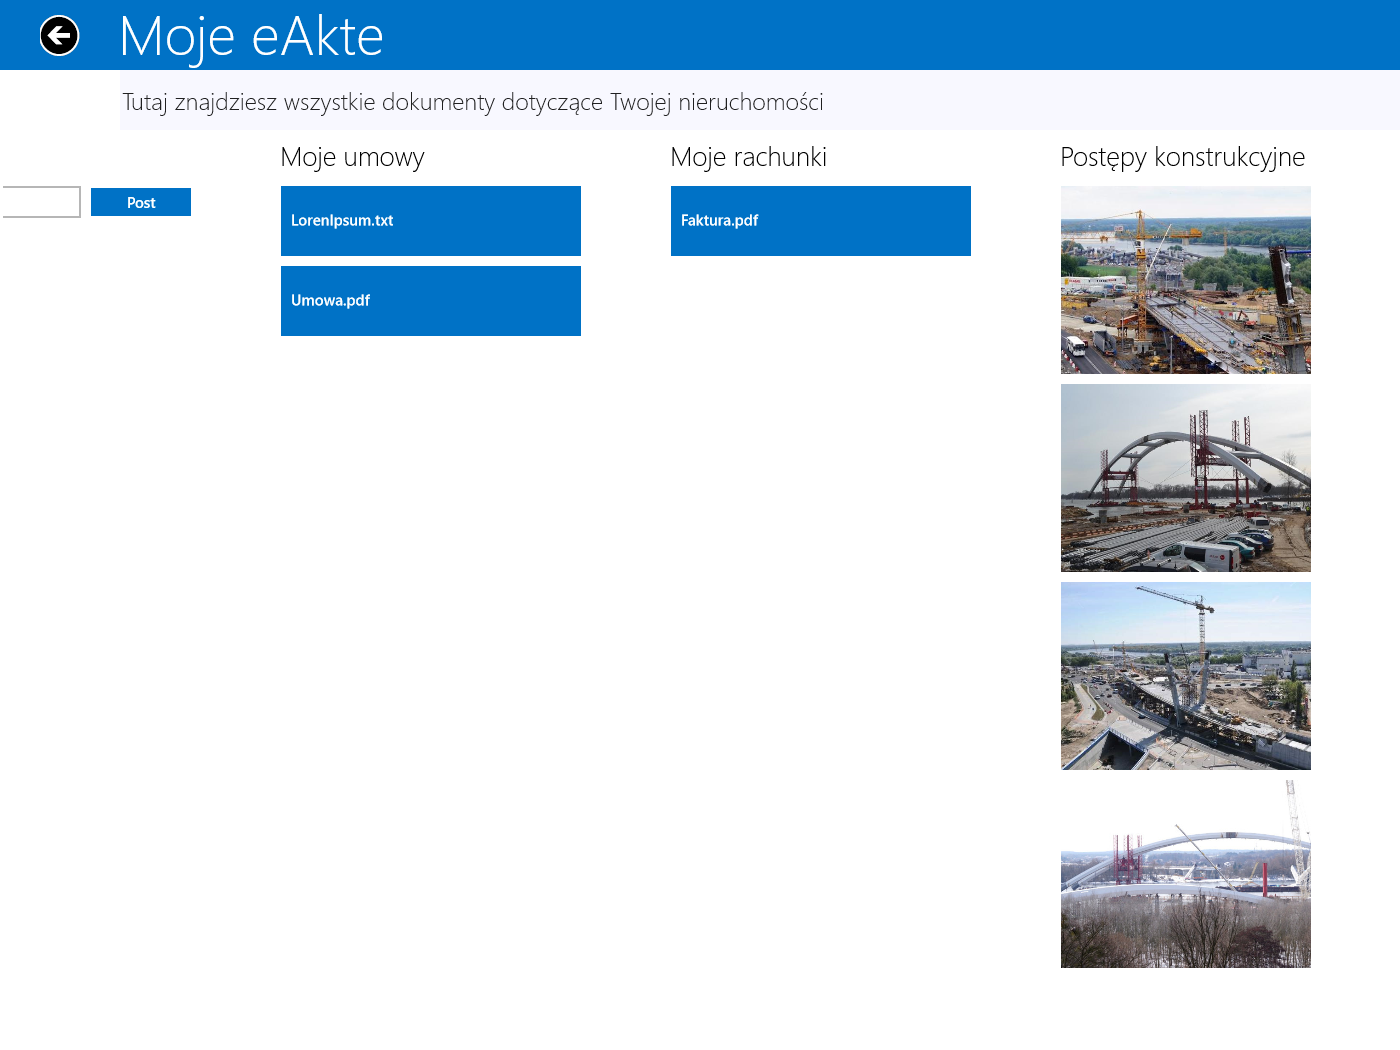
\includegraphics[width=\textwidth]{app_site}
\end{frame}

\begin{frame}[fragile]
\frametitle{Widok na plik}
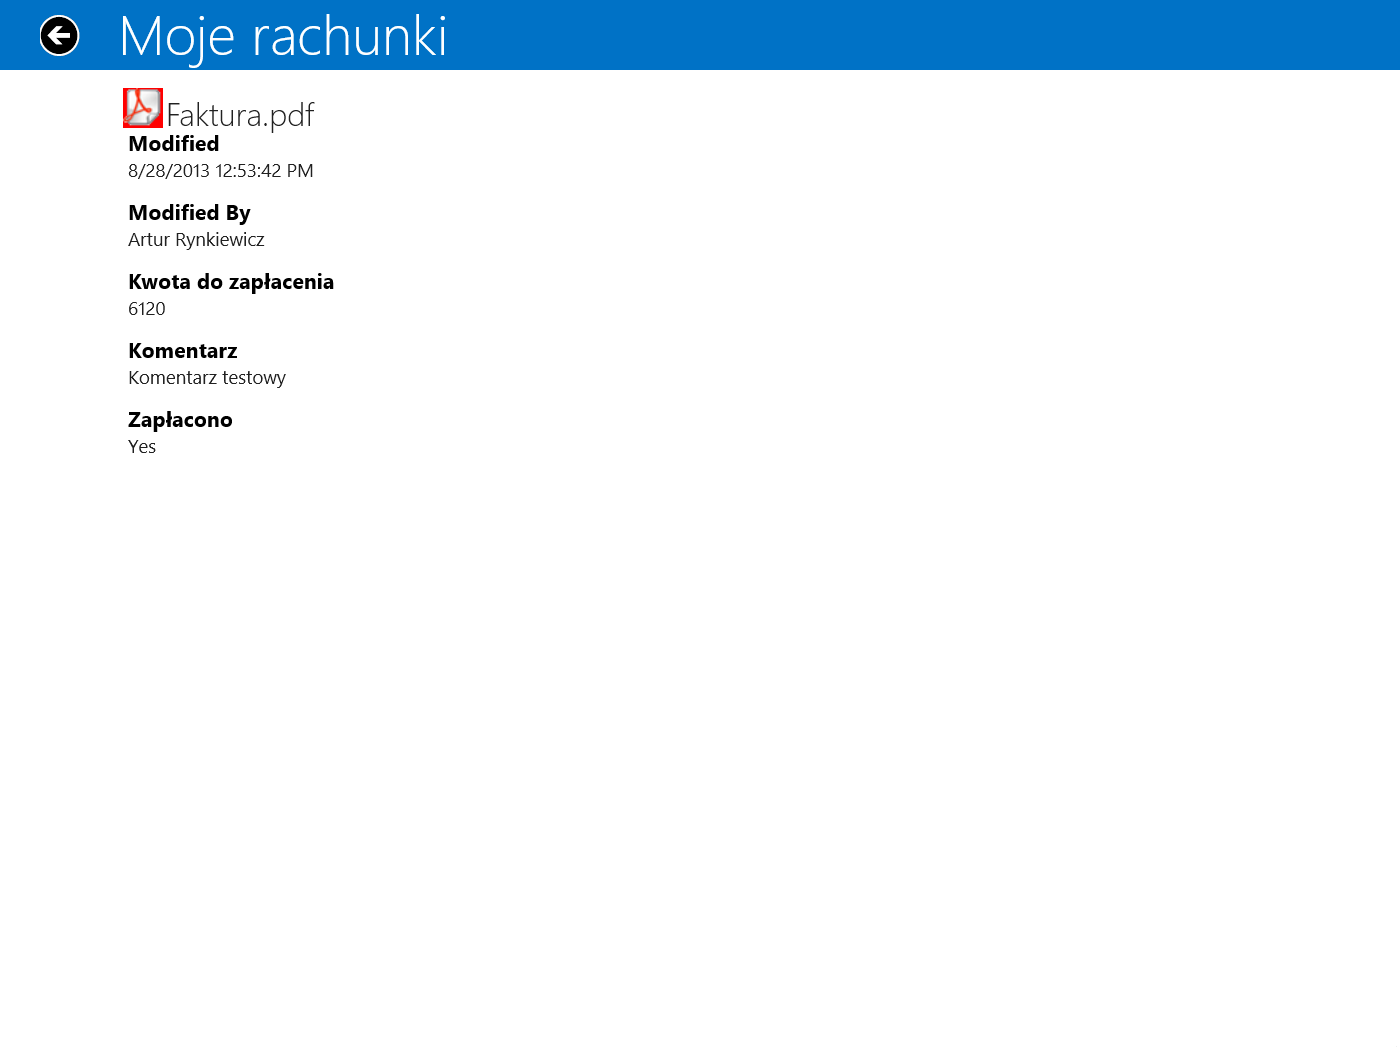
\includegraphics[width=\textwidth]{app_file}
\end{frame}

\begin{frame}[fragile]
\frametitle{Widok na obrazek}
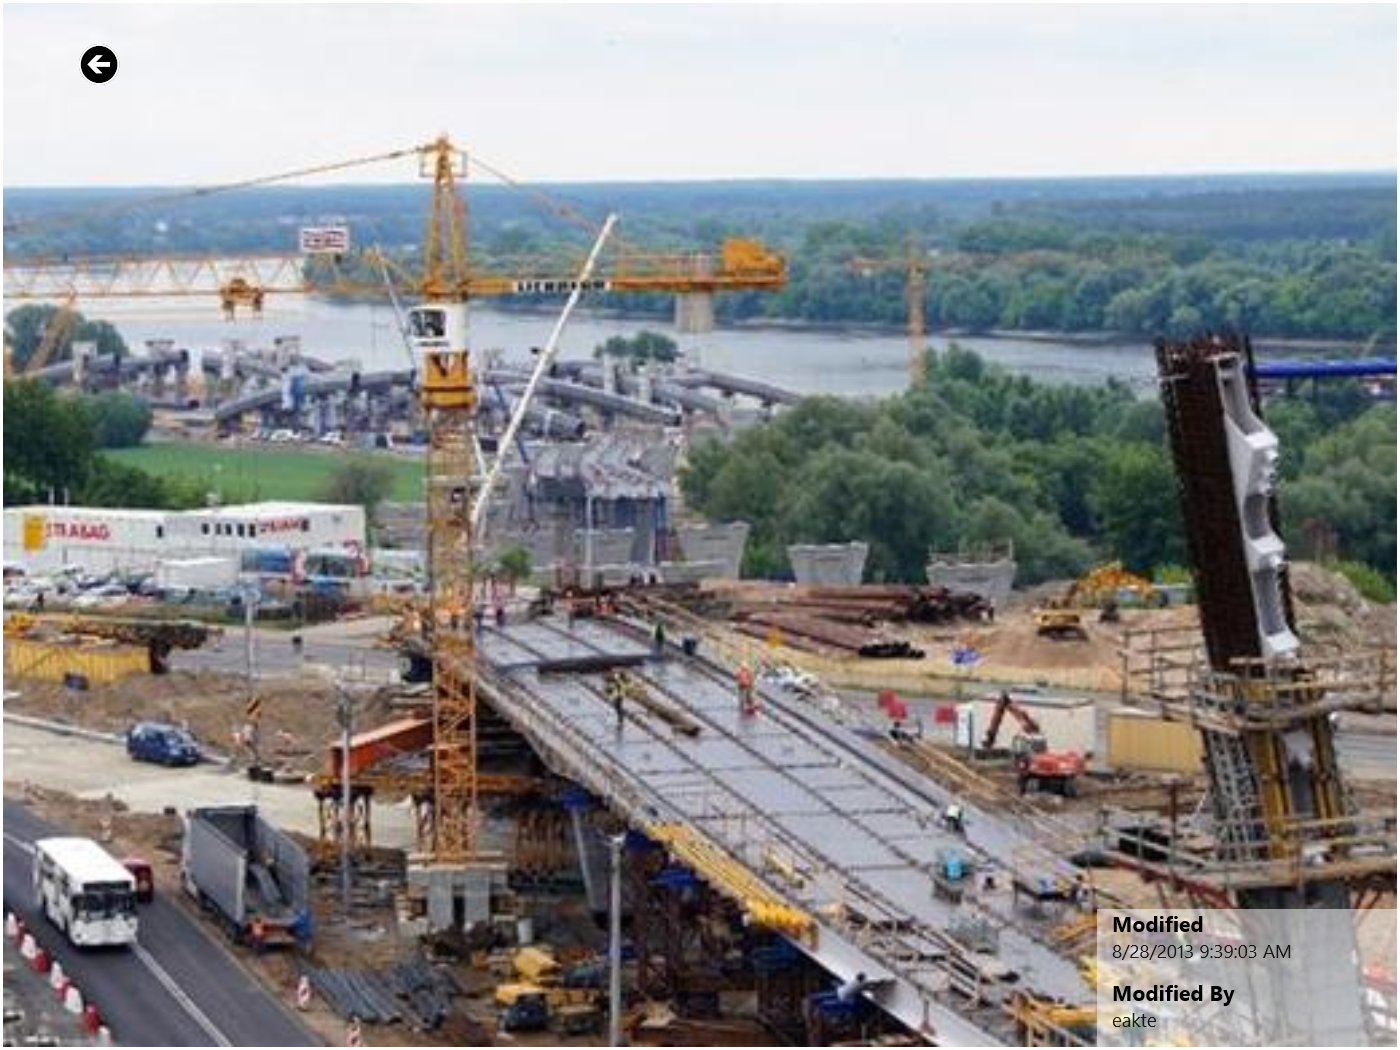
\includegraphics[width=\textwidth]{app_picture}
\end{frame}

\lstset{
  basicstyle=\ttfamily,
  columns=fullflexible,
  showstringspaces=false,
  commentstyle=\color{gray}\upshape
}

\begin{frame}[fragile]
\frametitle{Diagram przypadków użycia}
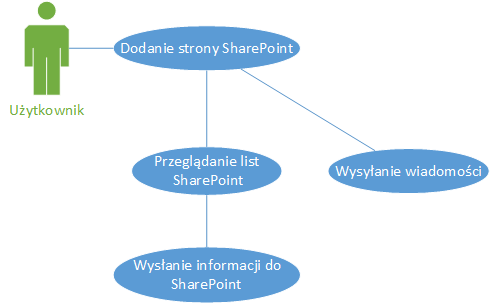
\includegraphics[scale=0.5]{example_usecase}
\end{frame}

\begin{frame}[fragile]
\frametitle{Model danych}
 \begin{adjustbox}{width=\textwidth}
\begin{lstlisting}[language=CSharp,basicstyle=\ttfamily]

public class List : BindableBase
{     
    [PrimaryKey, AutoIncrement]
    public int Idx { get; set; }    
	
    private string _title;
    public string Title
    {
        get { return _title; }
        set
        {
            SetProperty(ref _title, value);
        }
    }     
	
    private ObservableCollection<View> _views = new ObservableCollection<View>();
    [Ignore]
    public ObservableCollection<View> Views
    {
        get { return _views; }
        set
        {
            SetProperty(ref _views, value);                
        }
    }
}

\end{lstlisting}
\end{adjustbox}
\end{frame}

\begin{frame}[fragile]
\frametitle{Język \Csharp}
 \begin{adjustbox}{width=\textwidth}
\begin{lstlisting}[language=CSharp,basicstyle=\ttfamily]

private async void WriteTextButton_Click(object sender, RoutedEventArgs e) 
{ 
    try 
    {         
        StorageFile file = rootPage.sampleFile; 
        if (file != null) 
        { 
            string userContent = InputTextBox.Text; 
            if (!String.IsNullOrEmpty(userContent)) 
            { 
                await FileIO.WriteTextAsync(file, userContent); 
                OutputTextBlock.Text = "The following text was written to '"
                 + file.Name + "':" + Environment.NewLine 
                 + Environment.NewLine + userContent; 
            } 
            else 
            { 
                OutputTextBlock.Text = "The text box is empty, please write something and then click 'Write' again."; 
            } 
        } 
    } 
    catch (FileNotFoundException) 
    { 
        rootPage.NotifyUserFileNotExist(); 
    } 
} 
\end{lstlisting}
\end{adjustbox}
\end{frame}



\lstdefinelanguage{XML}
{
  morestring=[b]",
  morestring=[s]{>}{<},
  morecomment=[s]{<?}{?>},
  stringstyle=\color{black},
  identifierstyle=\color{darkblue},
  keywordstyle=\color{cyan},
  morekeywords={xmlns,version,type}% list your attributes here
}

\begin{frame}[fragile]
\frametitle{Widok aplikacji XAML}
 \begin{adjustbox}{width=\textwidth}
\begin{lstlisting}[language=XML,basicstyle=\ttfamily]

<Grid x:Name="LayoutRoot" Background="White" 
      HorizontalAlignment="Left" VerticalAlignment="Top"> 
        <Grid.RowDefinitions> 
            <RowDefinition Height="Auto"/> 
            <RowDefinition Height="*"/> 
        </Grid.RowDefinitions> 
        <Grid x:Name="Input" Grid.Row="0"> 
            <Grid.RowDefinitions> 
                <RowDefinition Height="Auto"/> 
                <RowDefinition Height="*"/> 
            </Grid.RowDefinitions> 
            <TextBlock x:Name="Scenario1Input"  TextWrapping="Wrap" 
            Grid.Row="0" Style="{StaticResource BasicTextStyle}" HorizontalAlignment="Left" > 
                Displays the profile information for the Internet Connection Profile. 
            </TextBlock> 
            <StackPanel Orientation="Horizontal" Margin="0,10,0,0" Grid.Row="1"> 
                <Button x:Name="InternetConnectionProfileButton" 
                Content="Get Internet Connection Profile Info" 
                Margin="0,0,10,0" Click="InternetConnectionProfile_Click"/> 
            </StackPanel> 
        </Grid> 
</Grid> 
\end{lstlisting}
\end{adjustbox}
\end{frame}


\begin{frame}[fragile]
\frametitle{Testy jednostkowe oraz TDD (Test Driven Development)}
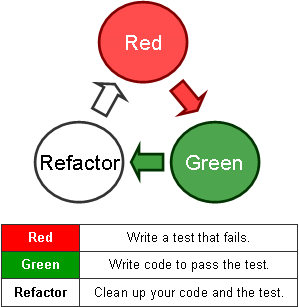
\includegraphics[scale=0.5]{tdd_cycle}
\end{frame}